\documentclass[journal]{IEEEtran}
\usepackage{cite}
\usepackage{amsmath,amssymb,amsfonts}
\usepackage{graphicx}
\usepackage{textcomp}
\usepackage{xcolor}
\usepackage{hyperref}
\usepackage{algorithm}
\usepackage{algpseudocode}

\hypersetup{
    colorlinks=true,
    linkcolor=blue,
    filecolor=magenta,      
    urlcolor=cyan,
}

\begin{document}

\title{Dynamic Hybrid Forecasting Models for Drug Consumption Prediction in Hospital Pharmacies}

\author{Yuxin Fan$^{*}$ and Siye Wu$^{\dagger}$ \\
$^{*}$School of Engineering and Applied Science, University of Pennsylvania, Canada, Toronto \\
Email: yuxinfan@alumni.upenn.edu \\
$^{\dagger}$Simon Business School, University of Rochester, Canada, Toronto \\
Email: april.siyewu@hotmail.com}

\maketitle

\begin{abstract}
Accurate and efficient drug consumption forecasting is crucial for hospital pharmacies to avoid overstocking, minimize wastage, and ensure continuous patient care. This study proposes a hybrid forecasting framework integrating XGBoost, Prophet, and SARIMAX to improve monthly consumption predictions at the drug-manufacturer level. Through rolling-window forecasting and advanced feature engineering, the proposed approach addresses challenges such as seasonality, trend shifts, and sparse data. Experimental results demonstrate significant improvements in prediction accuracy and robustness across diverse drug consumption scenarios.
\end{abstract}

\begin{IEEEkeywords}
Drug Consumption Forecasting, Hospital Pharmacies, Forecasting Models, XGBoost, Prophet, SARIMAX
\end{IEEEkeywords}

\section{Introduction}

Drug consumption forecasting plays a critical role in hospital pharmacy inventory management. Accurate predictions enable hospital pharmacies to ensure drug availability while minimizing costs associated with overstocking or stockouts. As highlighted by Koala et al.~\cite{koala2021factors}, forecasting drug consumption is particularly challenging due to numerous influencing factors, such as sociodemographic characteristics, morbidity patterns, drug price index, and seasonal factors like disease outbreaks or policy changes. This study aims to develop a hybrid forecasting framework tailored to address these challenges by integrating XGBoost, Prophet, and SARIMAX with rolling-window forecasting and advanced feature engineering.  

In previous studies, various forecasting techniques have been proposed to address one or more of these complexities. Taylor and Letham~\cite{taylor2018forecasting} introduce Prophet, a scalable forecasting method designed for large-scale applications, focusing on capturing general trends and seasonality with changepoint detection. However, Prophet is limited in handling external variables and often requires careful tuning to avoid overfitting to local patterns. Machine learning techniques, such as XGBoost proposed by Chen and Guestrin~\cite{chen2016xgboost}, effectively model non-linear relationships but struggle with sequential dependencies in time-series data. 

Furthermore, comparative and hybrid studies like those by Ferreira et al.~\cite{ferreira2018forecast} and Meng et al.~\cite{meng2021comparative} highlight that while LSTM improves non-linear pattern recognition compared to ARIMA and Prophet excels in handling sparse data, both face challenges with computational complexity and adaptability. Xu et al.~\cite{xu2019hybrid} demonstrate a hybrid approach combining linear regression and LSTM networks, which improves temporal forecasting but struggles with capturing complex, non-linear interactions across diverse datasets. Siddiqui et al.~\cite{siddiqui2021hybrid} explore hybrid models like ARIMA-Holt’s Winter, which improve upon traditional statistical methods but rely heavily on fixed architectures, limiting adaptability in dynamic environments. Rathipriya et al.~\cite{rathipriya2022pharma} utilize hybrid neural networks to address temporal patterns but face challenges with data sparsity and computational efficiency. 

In this study, to address the above limitations, our proposed framework introduces rolling-window forecasting to adjust predictions for non-stationary data and shifting trends dynamically, along with advanced feature engineering that enriches the data with lag features and trend indicators, capturing both short-term dependencies and long-term dynamics. These techniques are seamlessly integrated with hybrid complementary models: XGBoost, which models non-linear relationships and feature interactions; SARIMAX, which incorporates external variables and seasonality; and Prophet, which handles trend decomposition and missing data. This synergy provides a robust and versatile solution to the unique challenges of drug consumption forecasting, making the framework applicable across various drug types and manufacturers.

The remainder of this paper is organized as follows: Section II details the methodology, including data preprocessing and model design. Section III presents experimental results and discussions, highlighting the advantages of the proposed framework. Finally, Section IV concludes the study and outlines future research directions.

\section{Methodology}

\subsection{Introduction to Hybrid Model Framework}

The proposed hybrid forecasting framework integrates the complementary strengths of Prophet, SARIMAX, and XGBoost to address the challenges of drug consumption prediction. Unlike single-model approaches that are limited in their ability to generalize across diverse data characteristics, this framework leverages the distinct strengths of each model to provide more comprehensive and accurate predictions. By dynamically selecting the most appropriate model for each drug-manufacturer combination, the framework ensures that varying data patterns, including seasonal variations, non-linear dependencies, and sparse observations, are effectively captured.

A key challenge in drug consumption prediction is the variability in data characteristics across different drug-manufacturer combinations. Some datasets exhibit consistent and stable trends over time, while others may show significant volatility or sparsity. For example, drugs with high and regular demand may be well-suited to models like Prophet, which excels at decomposing long-term trends and seasonal components. Conversely, drugs with irregular consumption patterns or strong external influences may be better explained by SARIMAX, which incorporates external variables and captures short-term dynamics through advanced feature engineering. In cases where non-linear interactions and complex feature dependencies dominate, XGBoost is better equipped to model these relationships due to its gradient boosting mechanism and flexibility in feature selection.

To account for these differences, the framework evaluates each model’s performance on specific drug-manufacturer combinations using metrics such as R\(^2\) and symmetric mean absolute percentage error (SMAPE). These metrics provide a quantitative basis for selecting the model that best explains the underlying data patterns. For instance, a high R\(^2\) value indicates that a model effectively captures the variance in the data, while a low SMAPE suggests robust performance in capturing relative changes across time. By dynamically assigning the most suitable model to each combination, the framework maximizes prediction accuracy and minimizes the limitations associated with single-model approaches.

This model selection strategy highlights the heterogeneity in drug consumption trends and emphasizes the need for a hybrid approach. Drugs with stable and predictable behavior are efficiently handled by models like Prophet, while SARIMAX addresses datasets influenced by external factors or exhibiting strong seasonality. XGBoost complements these statistical models by providing superior accuracy for datasets with non-linear relationships or sparse observations. Through this collaborative mechanism, the hybrid framework not only enhances prediction robustness but also expands the scope of application to a wider variety of drug consumption scenarios.



\subsection{Model Design and Roles}

The hybrid forecasting framework integrates Prophet, SARIMAX, and XGBoost to leverage their respective strengths in addressing the challenges of drug consumption prediction. Each model is designed to fulfill a specific role, complementing the others to achieve higher accuracy and robustness. Prophet focuses on capturing long-term trends and seasonality, SARIMAX incorporates external variables and advanced feature engineering for short-term dependencies, and XGBoost models complex non-linear interactions among features. Together, they form a cohesive framework for dynamic and adaptive time-series forecasting.

\subsubsection{SARIMAX Model}

SARIMAX extends the traditional ARIMA model by incorporating external (exogenous) variables, allowing it to capture external influences on the target variable. This capability makes SARIMAX particularly suitable for time-series data with seasonality, trends, and additional contextual factors. The model is defined as:

\begin{equation}
y_{t} = \phi(B)\theta(B)^{-1} \left( c + \mathbf{X}_{t}\beta + \epsilon_{t} \right),
\end{equation}

where:
\begin{itemize}
    \item \(y_{t}\): The target variable (e.g., monthly drug consumption).
    \item \(\phi(B)\): The autoregressive (AR) operator.
    \item \(\theta(B)\): The moving average (MA) operator.
    \item \(c\): A constant term.
    \item \(\mathbf{X}_{t}\): A vector of exogenous variables at time \(t\).
    \item \(\beta\): The coefficient vector for \(\mathbf{X}_{t}\).
    \item \(\epsilon_{t}\): White noise error term.
\end{itemize}

To enhance prediction accuracy, SARIMAX incorporates various exogenous variables derived through advanced feature engineering. These include:

\text{Lagged values}:  
Lagged values capture the delayed effects of past consumption and are defined as:
\begin{equation}
\text{lag}_{k} = y_{t-k}, \quad k \in \{1, 3, 6, 12\}.
\end{equation}

\text{Rolling statistics}:  
Rolling statistics represent short-term trends and variability. They include the rolling mean and standard deviation:
\begin{equation}
\text{Rolling Mean}_{k} = \frac{1}{k} \sum_{i=1}^{k} y_{t-i},
\end{equation}
\begin{equation}
\text{Rolling Std}_{k} = \sqrt{\frac{1}{k} \sum_{i=1}^{k} (y_{t-i} - \text{Mean})^2}.
\end{equation}

\text{Exponential weighted moving average (EWMA)}:  
EWMA emphasizes recent observations with a smoothing factor \(\alpha\):
\begin{equation}
\text{EWMA}_{\alpha} = \alpha y_{t} + (1-\alpha) \cdot \text{EWMA}_{\alpha,t-1}.
\end{equation}

\text{Seasonality variables}:  
Monthly seasonality is encoded using trigonometric functions:
\begin{equation}
\text{Month\_sin} = \sin\left(\frac{2\pi \cdot \text{Month}}{12}\right),
\end{equation}
\begin{equation}
\text{Month\_cos} = \cos\left(\frac{2\pi \cdot \text{Month}}{12}\right).
\end{equation}

\text{Percentage change}:  
Percentage change measures relative variations over time:
\begin{equation}
\text{Pet\_Change}_{1} = \frac{y_{t} - y_{t-1}}{y_{t-1}},
\end{equation}
\begin{equation}
\text{Pet\_Change}_{3} = \frac{y_{t} - y_{t-3}}{y_{t-3}}.
\end{equation}

\text{Trend and volatility}:  
Trend strength captures long-term dynamics, while volatility measures variability:
\begin{equation}
\text{Trend Strength} = \frac{1}{k} \sum_{i=1}^{k} \lvert y_{t-i} - y_{t-i-1} \rvert,
\end{equation}
\begin{equation}
\text{Volatility} = \text{Rolling Std}_{k}.
\end{equation}

These exogenous variables, combined with SARIMAX’s inherent ability to model seasonality and trends, enable it to effectively capture complex temporal dependencies and improve prediction accuracy.

\subsubsection{XGBoost Model}

XGBoost is a gradient boosting framework designed to construct an ensemble of decision trees for predicting target variables. Its ability to capture non-linear relationships and complex interactions among features makes it highly effective for time-series forecasting tasks, particularly in scenarios involving dynamic patterns and sparse data. The model predicts the target variable \(y_t\) through an additive function:

\begin{equation}
\hat{y}_{t} = F(x_{t}) = \sum_{k=1}^{K} f_{k}(x_{t}), \quad f_{k} \in \mathcal{F},
\end{equation}

where \(\hat{y}_{t}\) is the predicted value at time \(t\), \(x_{t}\) represents the input features, \(f_{k}\) denotes the \(k\)-th decision tree, and \(\mathcal{F}\) is the function space of decision trees.

The predictive power of XGBoost in this framework is enhanced through careful feature engineering. Temporal dependencies are captured by incorporating lagged values, such as historical consumption data (\(y_{t-1}, y_{t-2}, \dots, y_{t-k}\)), which model delayed effects of past consumption. Rolling statistics, including moving averages and standard deviations over defined windows (e.g., 3, 6, and 12 periods), are introduced to quantify local trends and variability. Seasonal patterns are encoded using trigonometric functions (\(\sin\) and \(\cos\)) to capture monthly or quarterly cycles, and interaction terms are derived to represent the interplay between lagged values and seasonal indicators. This comprehensive feature set enables XGBoost to model both short-term fluctuations and long-term patterns effectively.

To address the non-stationarity inherent in time-series data, the model is trained iteratively using a rolling-window approach. At each iteration, the training dataset is updated to include the most recent observations while maintaining a fixed window size. The model is then retrained on this updated dataset, and predictions are made for the subsequent time step. This rolling-window strategy ensures that the model dynamically adapts to evolving trends and minimizes the risk of overfitting to older data.

Hyperparameter optimization plays a crucial role in maximizing the model’s performance. During each training iteration, a grid search is conducted to tune parameters such as the number of estimators, learning rate, maximum tree depth, subsample ratio, and column sampling ratio. The number of estimators determines the size of the ensemble, while the learning rate controls the contribution of each tree to the final prediction. Maximum tree depth limits the complexity of individual trees to prevent overfitting, and the subsample and column sampling ratios regulate the fraction of data and features used for training, enhancing the model’s generalization capability.

XGBoost serves as a critical component of the hybrid forecasting framework by complementing the strengths of statistical models like SARIMAX. Its ability to model non-linear interactions and complex dependencies allows it to address challenges posed by irregular patterns and sparse data. Moreover, its integration with rolling-window training and advanced feature engineering ensures robustness and adaptability, making it a valuable tool for predicting drug consumption trends in diverse scenarios.


\subsubsection{Prophet Model}

Prophet is a robust time-series forecasting model developed by Facebook, designed to explicitly decompose time-series data into trend, seasonality, and holiday components. Its ability to handle missing values, outliers, and irregular patterns makes it particularly suitable for real-world applications involving complex and dynamic data. The model predicts the target variable \(y_t\) as:

\begin{equation}
y_{t} = g(t) + s(t) + h(t) + \epsilon_{t},
\end{equation}

where \(g(t)\) represents the long-term trend, \(s(t)\) models recurring seasonal patterns using Fourier series, \(h(t)\) accounts for holiday effects or special events, and \(\epsilon_{t}\) is a white noise error term. This decomposition framework allows Prophet to capture distinct components of time-series data independently, providing interpretable results while maintaining high predictive accuracy.

To ensure the model's adaptability to different drug-manufacturer combinations, key hyperparameters are optimized through grid search. These parameters include:
- \textit{seasonality\_mode}, which determines whether seasonal patterns are modeled as additive or multiplicative effects;
- \textit{changepoint\_prior\_scale}, controlling the flexibility of the trend component by determining the likelihood of abrupt changes in growth;
- \textit{seasonality\_prior\_scale}, which adjusts the weight assigned to seasonal components.

The grid search systematically explores combinations of these hyperparameters, enabling the model to identify configurations that best capture the temporal dynamics of drug consumption. For example, a higher \textit{changepoint\_prior\_scale} allows the model to adapt to datasets with frequent structural changes in trend, while a lower value favors smoother transitions.

Prophet’s rolling-window forecasting strategy further enhances its robustness. By iteratively retraining the model on the most recent data, the framework dynamically incorporates emerging trends and minimizes the impact of outdated patterns. This approach, combined with the model's inherent decomposition capabilities, ensures accurate and interpretable predictions, even for datasets with irregular or sparse observations.

\subsection{Dynamic Rolling-Window Forecasting}

Time-series data often exhibit non-stationarity, where patterns such as trends, seasonality, and noise evolve over time. Static forecasting approaches, which rely on fixed historical data, may fail to adequately capture these dynamics, leading to suboptimal performance. To address this challenge, a dynamic rolling-window forecasting strategy is employed in this study, enabling the models to adaptively update their predictions by leveraging the most recent information.

The rolling-window mechanism operates iteratively. At each time step \(t\), the training dataset is updated to include the most recent observations while discarding older data beyond the defined window size. This dynamic adjustment ensures that the models prioritize recent patterns, which are often more predictive of future behavior, while mitigating the influence of outdated or less relevant data. Formally, the training dataset at time \(t\) can be expressed as:

\[
\mathcal{D}_{t} = \{(y_{\tau}, \mathbf{X}_{\tau}) \mid \tau \in [t - W, t-1]\},
\]

where \(\mathcal{D}_{t}\) represents the dataset used for training at time \(t\), \(W\) is the window size, \(y_{\tau}\) denotes the target variable, and \(\mathbf{X}_{\tau}\) encompasses the corresponding feature vectors. After training on \(\mathcal{D}_{t}\), predictions are generated for the next time step (\(t+1\)).

This strategy is particularly advantageous for capturing short-term dynamics in non-stationary data. By continuously updating the training window, the models are able to respond to structural changes in the data, such as shifts in trends or seasonal patterns. Furthermore, the rolling-window approach inherently supports the detection of emerging behaviors, ensuring that the forecasting framework remains robust in dynamic and evolving environments.

A critical consideration in rolling-window forecasting is the determination of an appropriate window size (\(W\)). A larger \(W\) incorporates long-term historical information, which may benefit datasets with persistent trends or pronounced seasonality. Conversely, a smaller \(W\) focuses on recent observations, offering greater sensitivity to abrupt changes or irregular patterns. To balance these trade-offs, this study empirically evaluates multiple window sizes for each model and selects the optimal configuration based on performance metrics such as root mean squared error (RMSE) and symmetric mean absolute percentage error (SMAPE).

The integration of rolling-window forecasting into the hybrid framework further enhances its adaptability. For example, SARIMAX dynamically recalibrates its coefficients using the updated dataset, allowing it to effectively model short-term dependencies and external influences. Similarly, XGBoost leverages the rolling-window mechanism to refine its decision trees, incorporating the most recent feature interactions to capture evolving non-linear relationships. Prophet, with its inherent trend decomposition capabilities, also benefits from the dynamic updating of its training set, ensuring that its predictions remain aligned with the latest trends.

In summary, the dynamic rolling-window forecasting strategy underpins the robustness and flexibility of the proposed framework. By iteratively incorporating recent information while adapting to structural changes, this approach ensures that the models remain both responsive and resilient, achieving superior forecasting performance across diverse drug consumption scenarios.

\section{Experiments}

\subsection{Dataset}
The dataset used in this study consists of monthly drug consumption records collected from various hospital pharmacies between January 1, 2018, and September 1, 2024. The data include a diverse range of drugs across multiple categories and manufacturers, ensuring a comprehensive representation of pharmaceutical demand. Each record contains the drug name, manufacturer, monthly consumption values, inventory levels, and associated features such as proportions and trends. This dataset provides a robust foundation for developing and testing the proposed forecasting framework.

\subsection{Data Processing}
A comprehensive preprocessing pipeline was applied to ensure data quality and consistency, while focusing on key steps relevant to our framework. Missing values in critical features were interpolated where possible, and records with excessive missing data were excluded to maintain dataset integrity.

Outliers in consumption data were addressed using a rolling-window approach. For each drug-manufacturer combination, rolling statistics such as mean and standard deviation were computed over a seven-month window. Values exceeding three standard deviations from the mean or falling outside the 5th and 95th percentiles were flagged as anomalies and adjusted to boundary values to preserve the time series' continuity.

To ensure the dataset included only high-quality samples for modeling, groups with fewer than six months of non-zero consumption data or those exhibiting extreme sparsity were excluded. Temporal autocorrelation of consumption data was assessed, and groups failing to exhibit sufficient autocorrelation were removed. Additional filtering criteria included variance thresholds and limits on skewness to avoid heavily imbalanced target distributions.

Feature engineering was performed to enhance the dataset's predictive power. Derived features such as lagged consumption values (e.g., previous month’s consumption), rolling statistics (e.g., mean, variance, and percent changes), and seasonality indicators encoded with trigonometric functions were created to capture temporal dependencies and periodic trends. These steps ensured that the final dataset was robust, informative, and well-suited for downstream predictive modeling tasks.


\subsection{Experimental Setup}
Models are evaluated using the following metrics:
\begin{enumerate}
    \item \textbf{Root Mean Squared Error (RMSE)}:
    \begin{equation}
    \text{RMSE}=\sqrt{\frac{1}{n}\sum_{i=1}^{n}(y_{i}-\hat{y}_{i})^{2}}.
    \end{equation}

    \item \textbf{Mean Absolute Error (MAE)}:
    \begin{equation}
    \text{MAE}=\frac{1}{n}\sum_{i=1}^{n}|y_{i}-\hat{y}_{i}|\,.
    \end{equation}

    \item \textbf{Symmetric Mean Absolute Percentage Error (SMAPE)}:
    \begin{equation}
    \text{SMAPE}=\frac{1}{n}\sum_{i=1}^{n}\frac{|y_{i}-\hat{y}_{i}|}{\frac{|y_{i}|+|\hat{y}_{i}|}{2}}\times 100\%, \quad \text{where}\ |y_{i}| + |\hat{y}_{i}| > 0.
    \end{equation}
    Here, cases where the denominator is zero are excluded.

    \item \textbf{Coefficient of Determination (Weighted R²)}:
    \begin{equation}
    R^{2}=1-\frac{\sum_{i=1}^{n}(y_{i}-\hat{y}_{i})^{2}}{\sum_{i=1}^{n}(y_{i}-\bar{y})^{2}},
    \end{equation}
    where \( \bar{y} \) is the mean of the actual values.
\end{enumerate}


\subsection{Data Analysis}

To evaluate the effectiveness of different forecasting models, we considered three state-of-the-art techniques: SARIMAX, Prophet, and XGBoost. Each model was applied to forecast sales data for a diverse set of drugs and manufacturers. The dataset consisted of weekly time series data spanning multiple years, capturing trends, seasonality, and irregular fluctuations in sales. Key metrics such as $R^2$, RMSE (Root Mean Squared Error), MAE (Mean Absolute Error), and SMAPE (Symmetric Mean Absolute Percentage Error) were used to assess model performance.

The selection of the optimal model for each drug-manufacturer pair was based on achieving the highest $R^2$ and minimizing RMSE, MAE, and SMAPE. The results highlighted that no single model universally outperformed the others across all cases, underscoring the importance of tailoring the choice of forecasting models to specific data characteristics. SARIMAX excelled in capturing seasonality and long-term trends, while XGBoost demonstrated strong performance in handling non-linear relationships. Prophet, designed for business forecasting, performed well in cases with prominent seasonality.

\subsection{Model Results}

\subsubsection{Representative Drug Cases}

\paragraph{XGBoost Model} % 确保 XGBoost、Prophet 和 SARIMAX 平行
\begin{itemize}
\item \textbf{Drug:} Mycophenolate Sodium Enteric Tablets
\begin{itemize}
\item \textbf{Manufacturer:} Novartis Switzerland
\item \textbf{Metrics:} $R^2 = 0.8154$, RMSE = 243.21, MAE = 155.63, SMAPE = 25.40
\end{itemize}
XGBoost showed exceptional performance for this drug by effectively capturing the complex non-linear patterns and sudden changes in demand, particularly evident in the volatile periods of 2018-2020.
\begin{figure}[H]
\centering
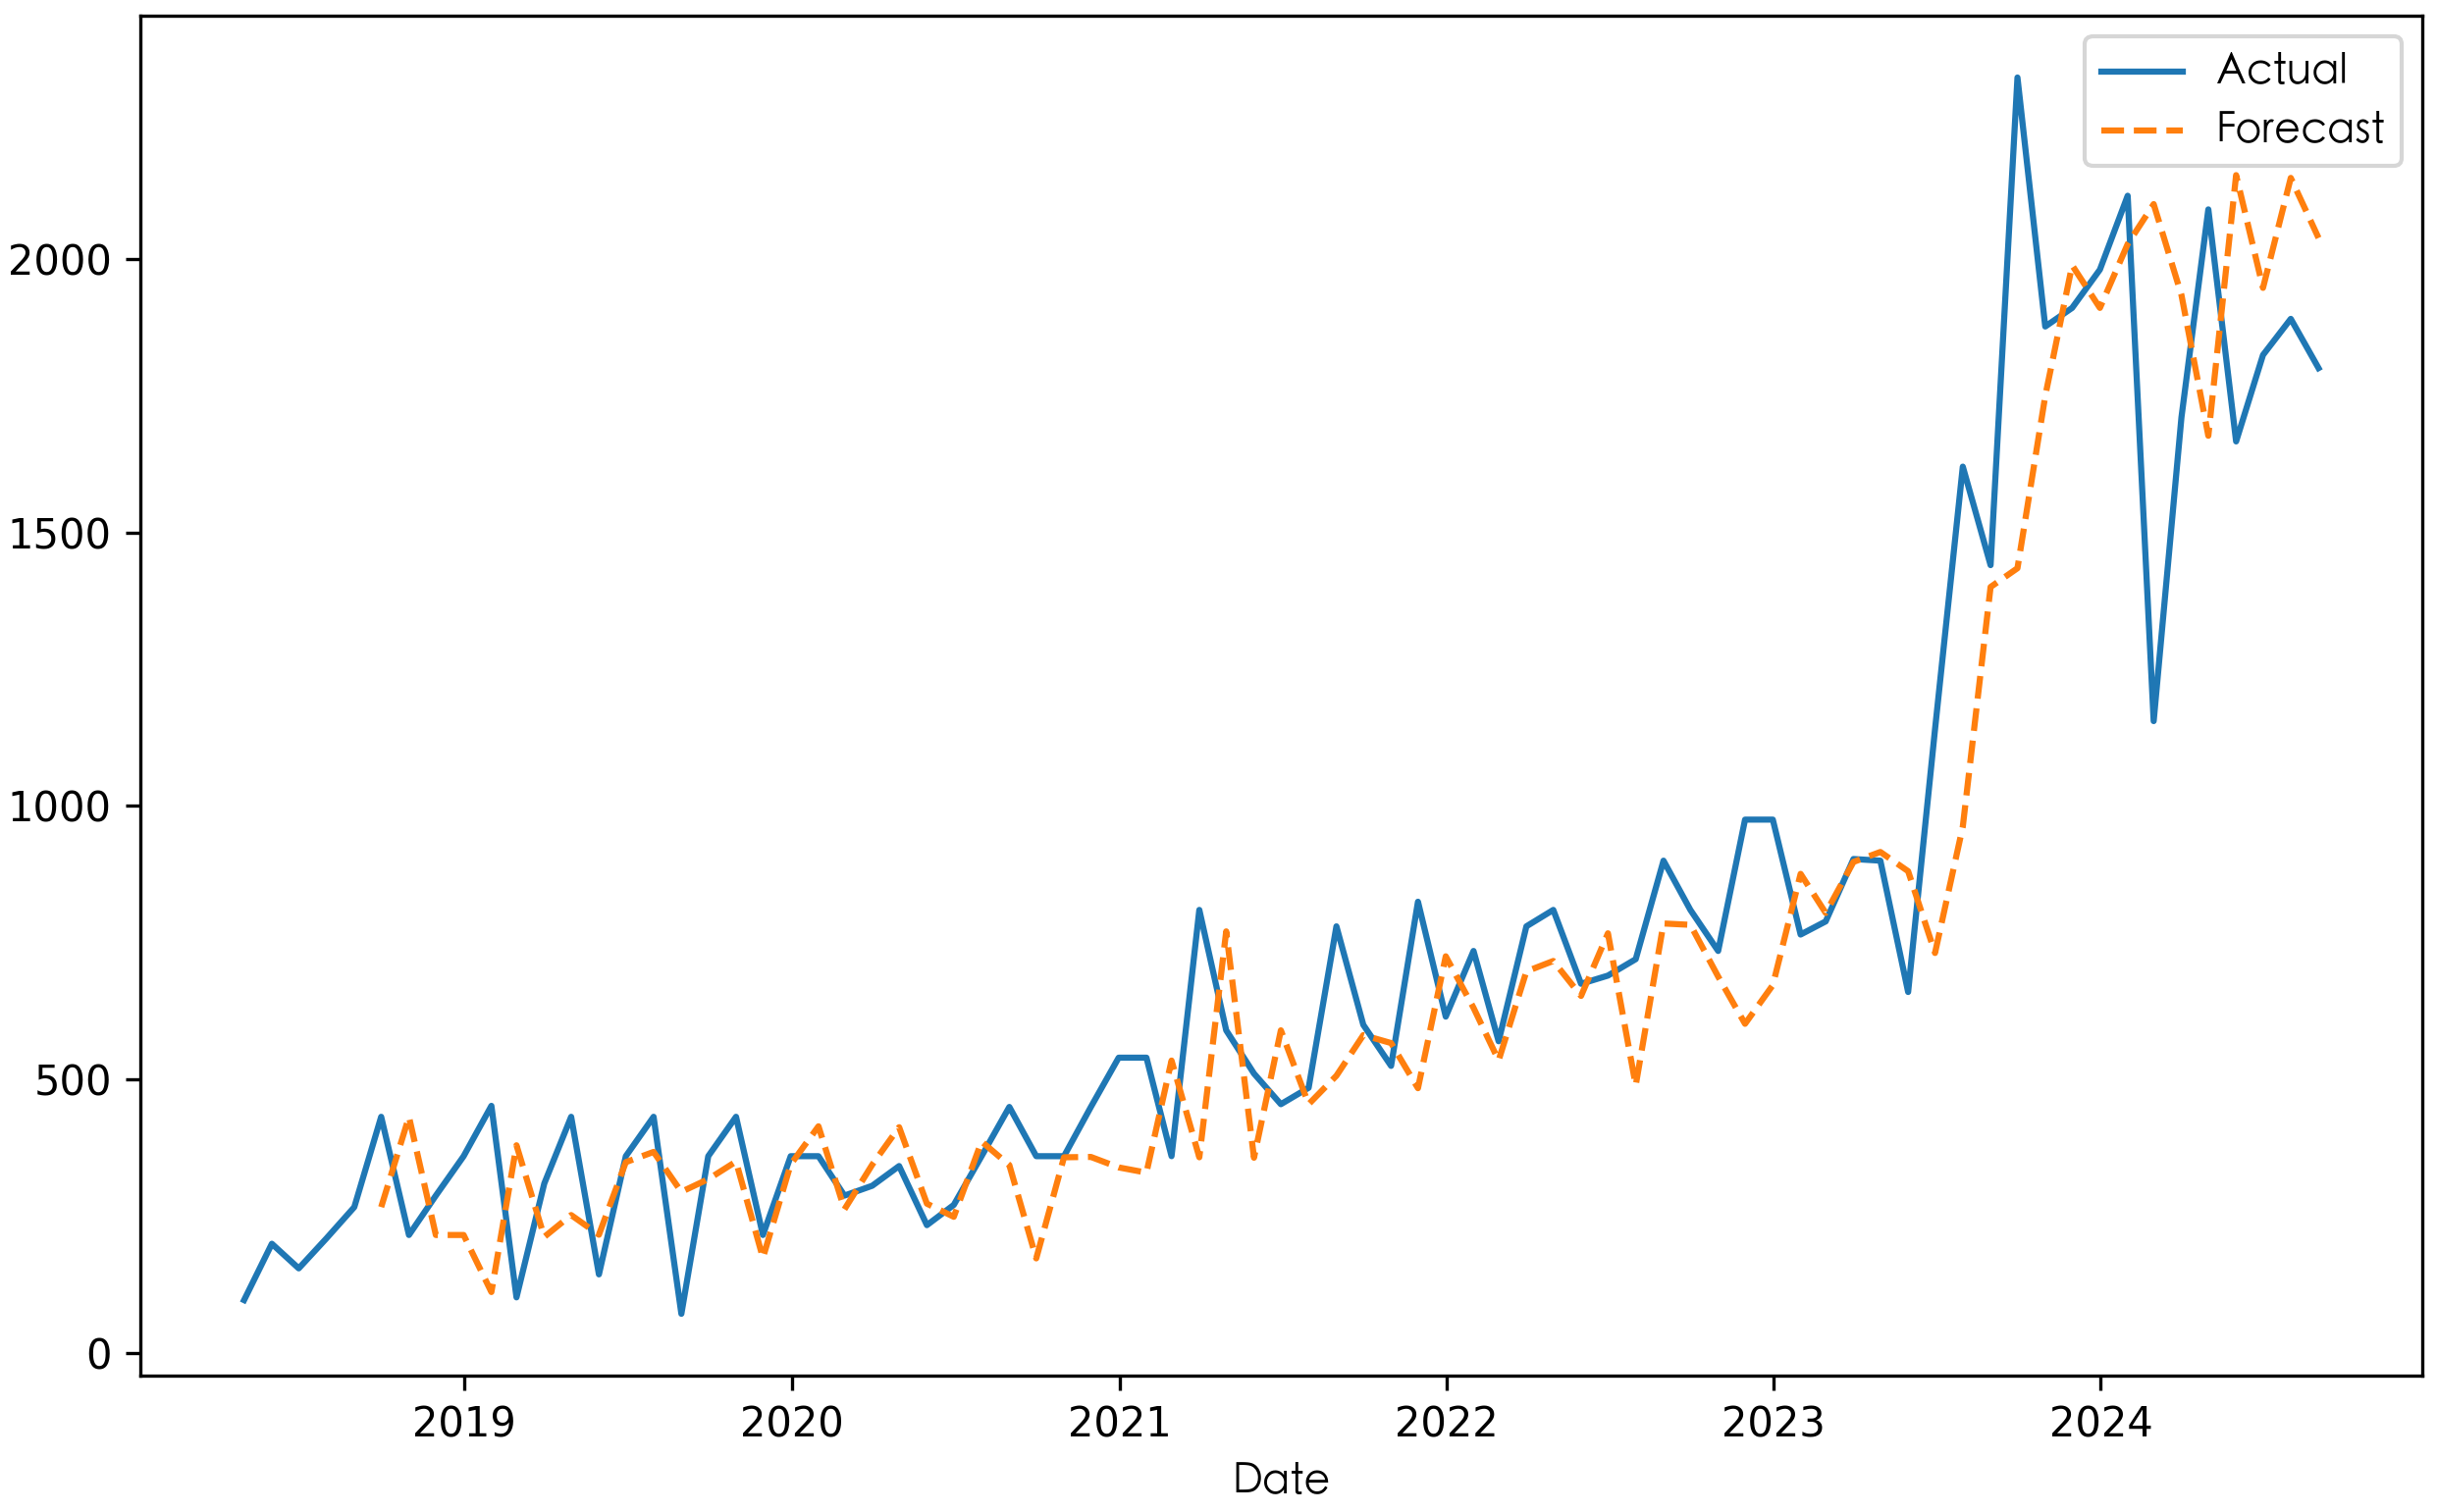
\includegraphics[width=\linewidth]{/Users/aprilwu/Desktop/Result_Paper/XGBoost_Prediction_麦考酚钠肠溶片_瑞士诺华.png}
\caption{XGBoost Prediction for Mycophenolate Sodium Enteric Tablets by Novartis.}
\label{fig:mycophenolate}
\end{figure}
\item \textbf{Drug:} Flurbiprofen Gel Patch
\begin{itemize}
\item \textbf{Manufacturer:} Jingtaide
\item \textbf{Metrics:} $R^2 = 0.7902$, RMSE = 1161.72, MAE = 699.53, SMAPE = 21.14
\end{itemize}
XGBoost effectively handled the increasing trend and high volatility in sales, demonstrating its strength in capturing complex patterns and sudden market changes.
\begin{figure}[H]
\centering
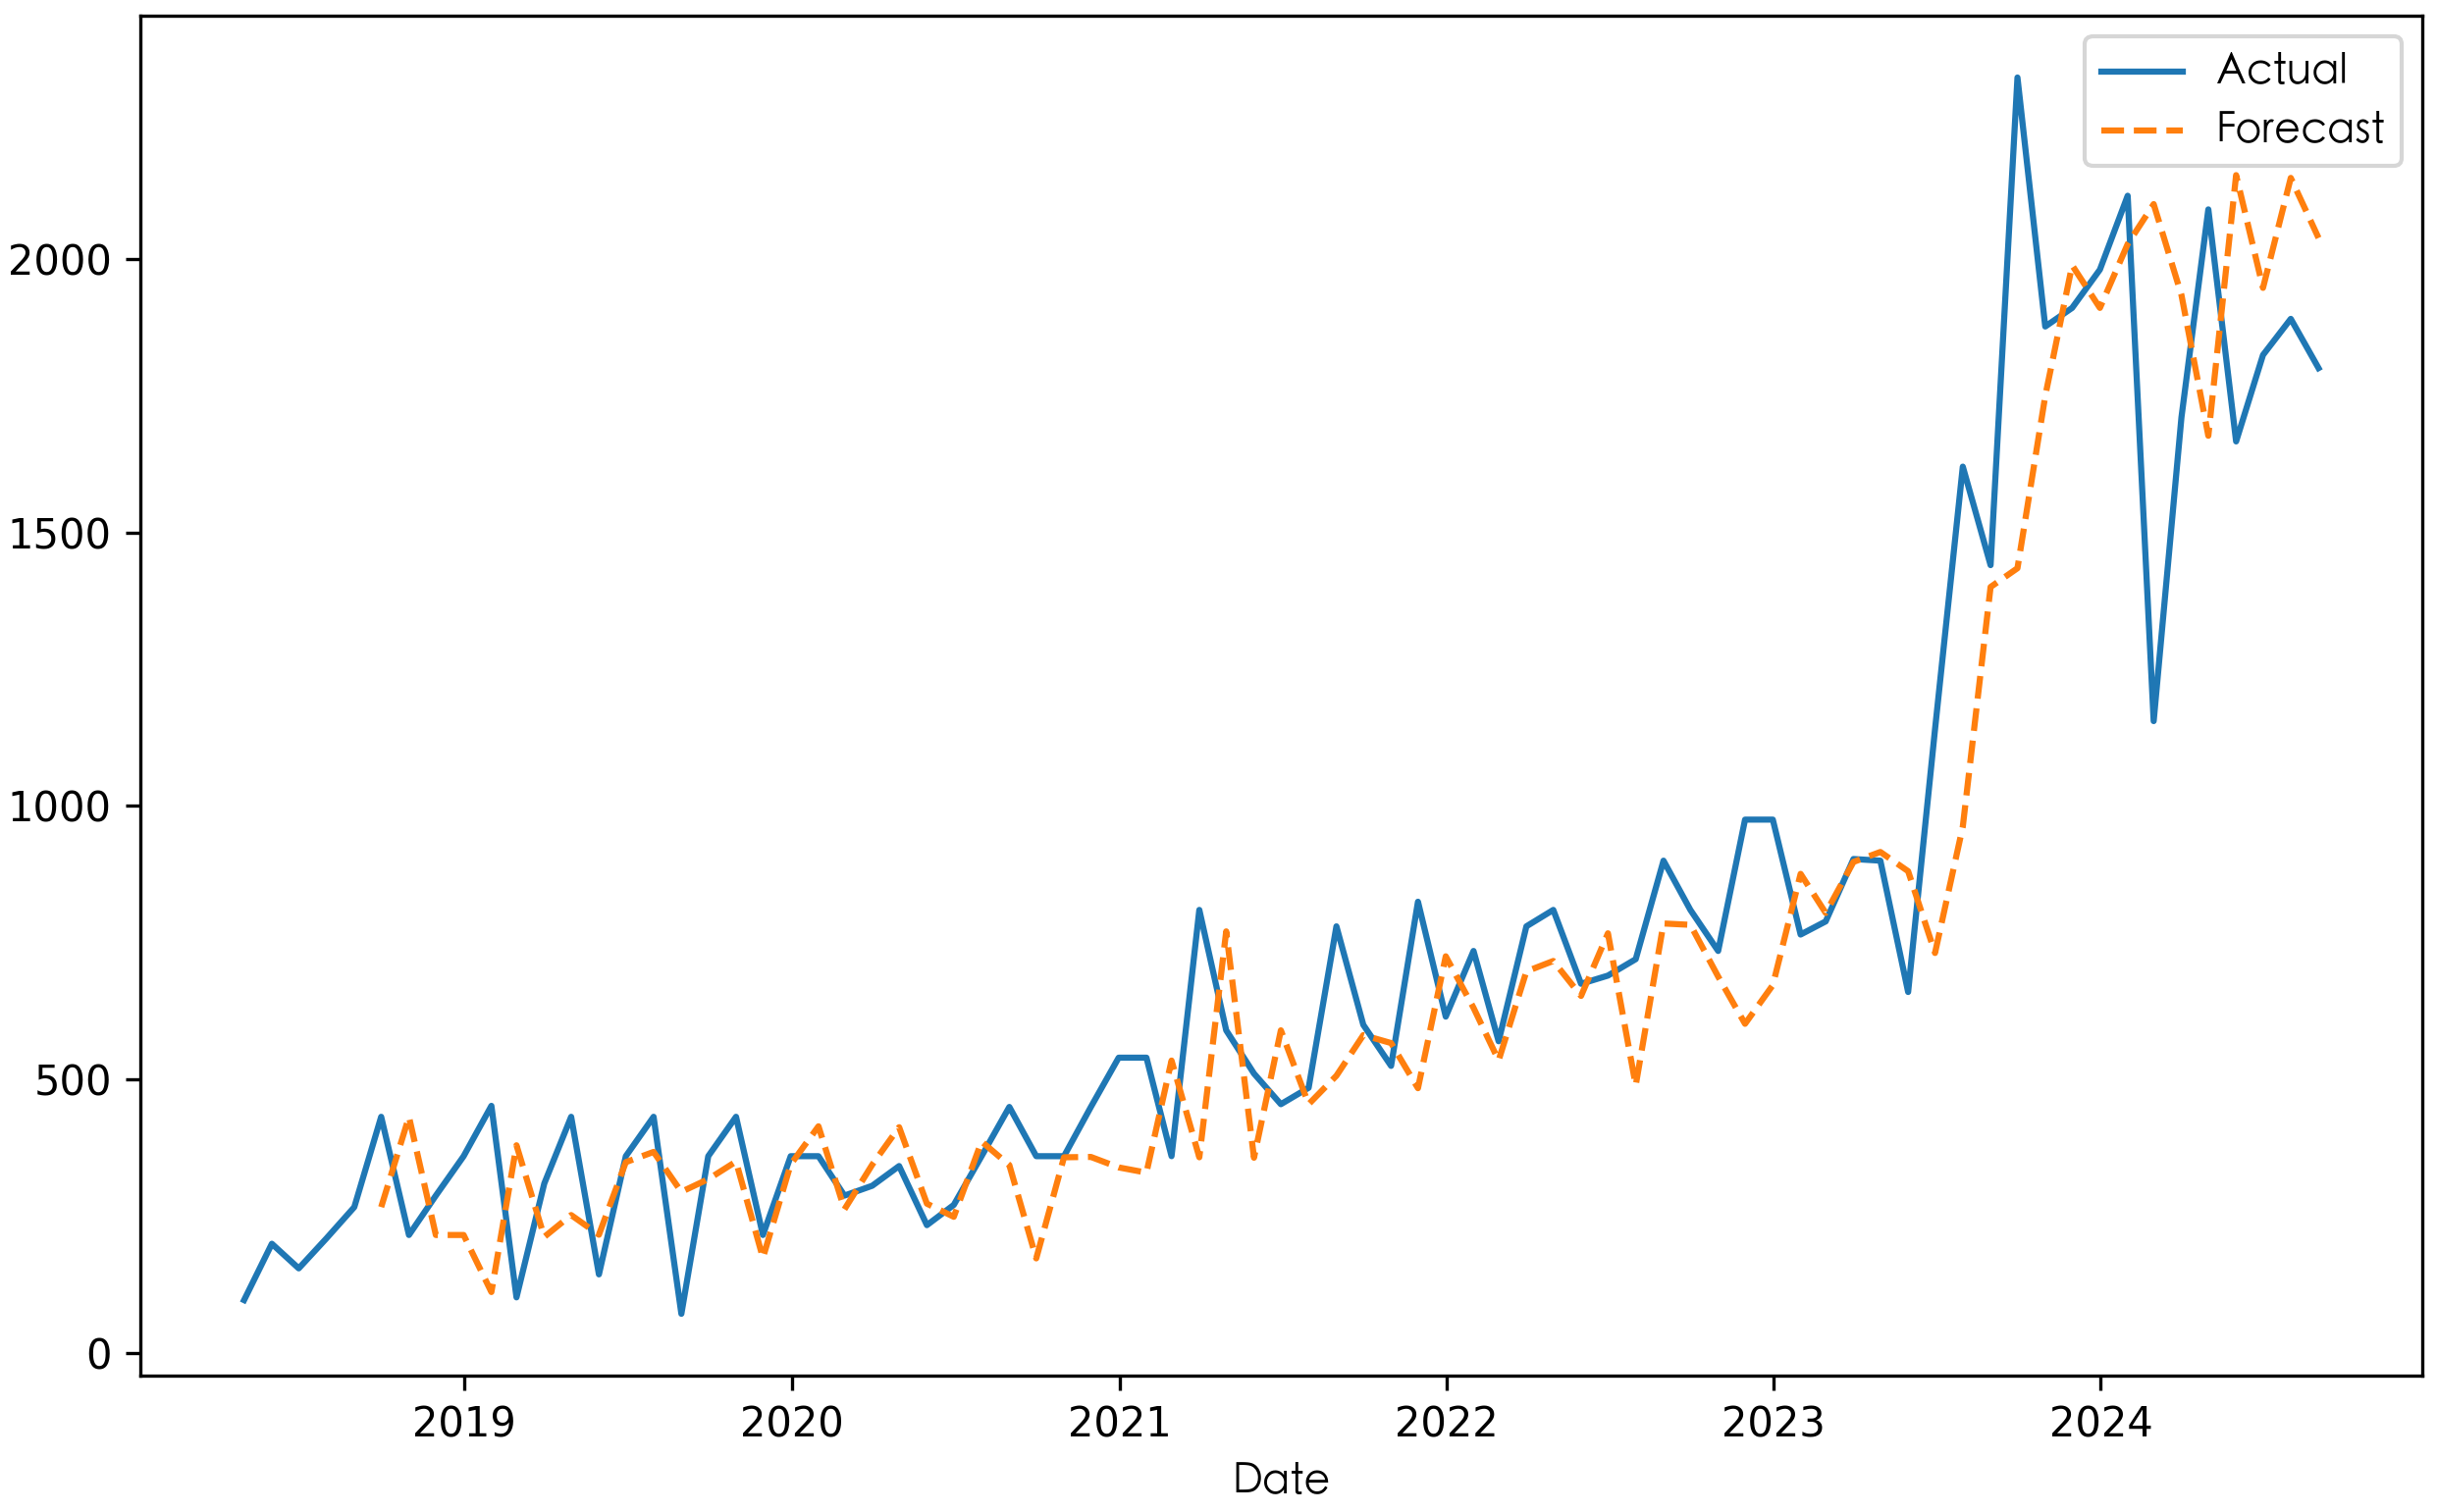
\includegraphics[width=\linewidth]{/Users/aprilwu/Desktop/Result_Paper/XGBoost_Prediction_麦考酚钠肠溶片_瑞士诺华.png}
\caption{XGBoost Prediction for Flurbiprofen Gel Patch by Jingtaide.}
\label{fig:flurbiprofen}
\end{figure}
\end{itemize}

\paragraph{Prophet Model}
\begin{itemize}
\item \textbf{Drug:} Compound Phellodendron Liquid
\begin{itemize}
\item \textbf{Manufacturer:} Lu Hanfang
\item \textbf{Metrics:} $R^2 = 0.7898$, RMSE = 1057.92, MAE = 735.55, SMAPE = 22.63
\end{itemize}
Prophet excelled in modeling this drug's sales pattern due to its robust handling of trend changes and seasonal variations, particularly evident in the steady growth pattern.
\begin{figure}[H]
\centering
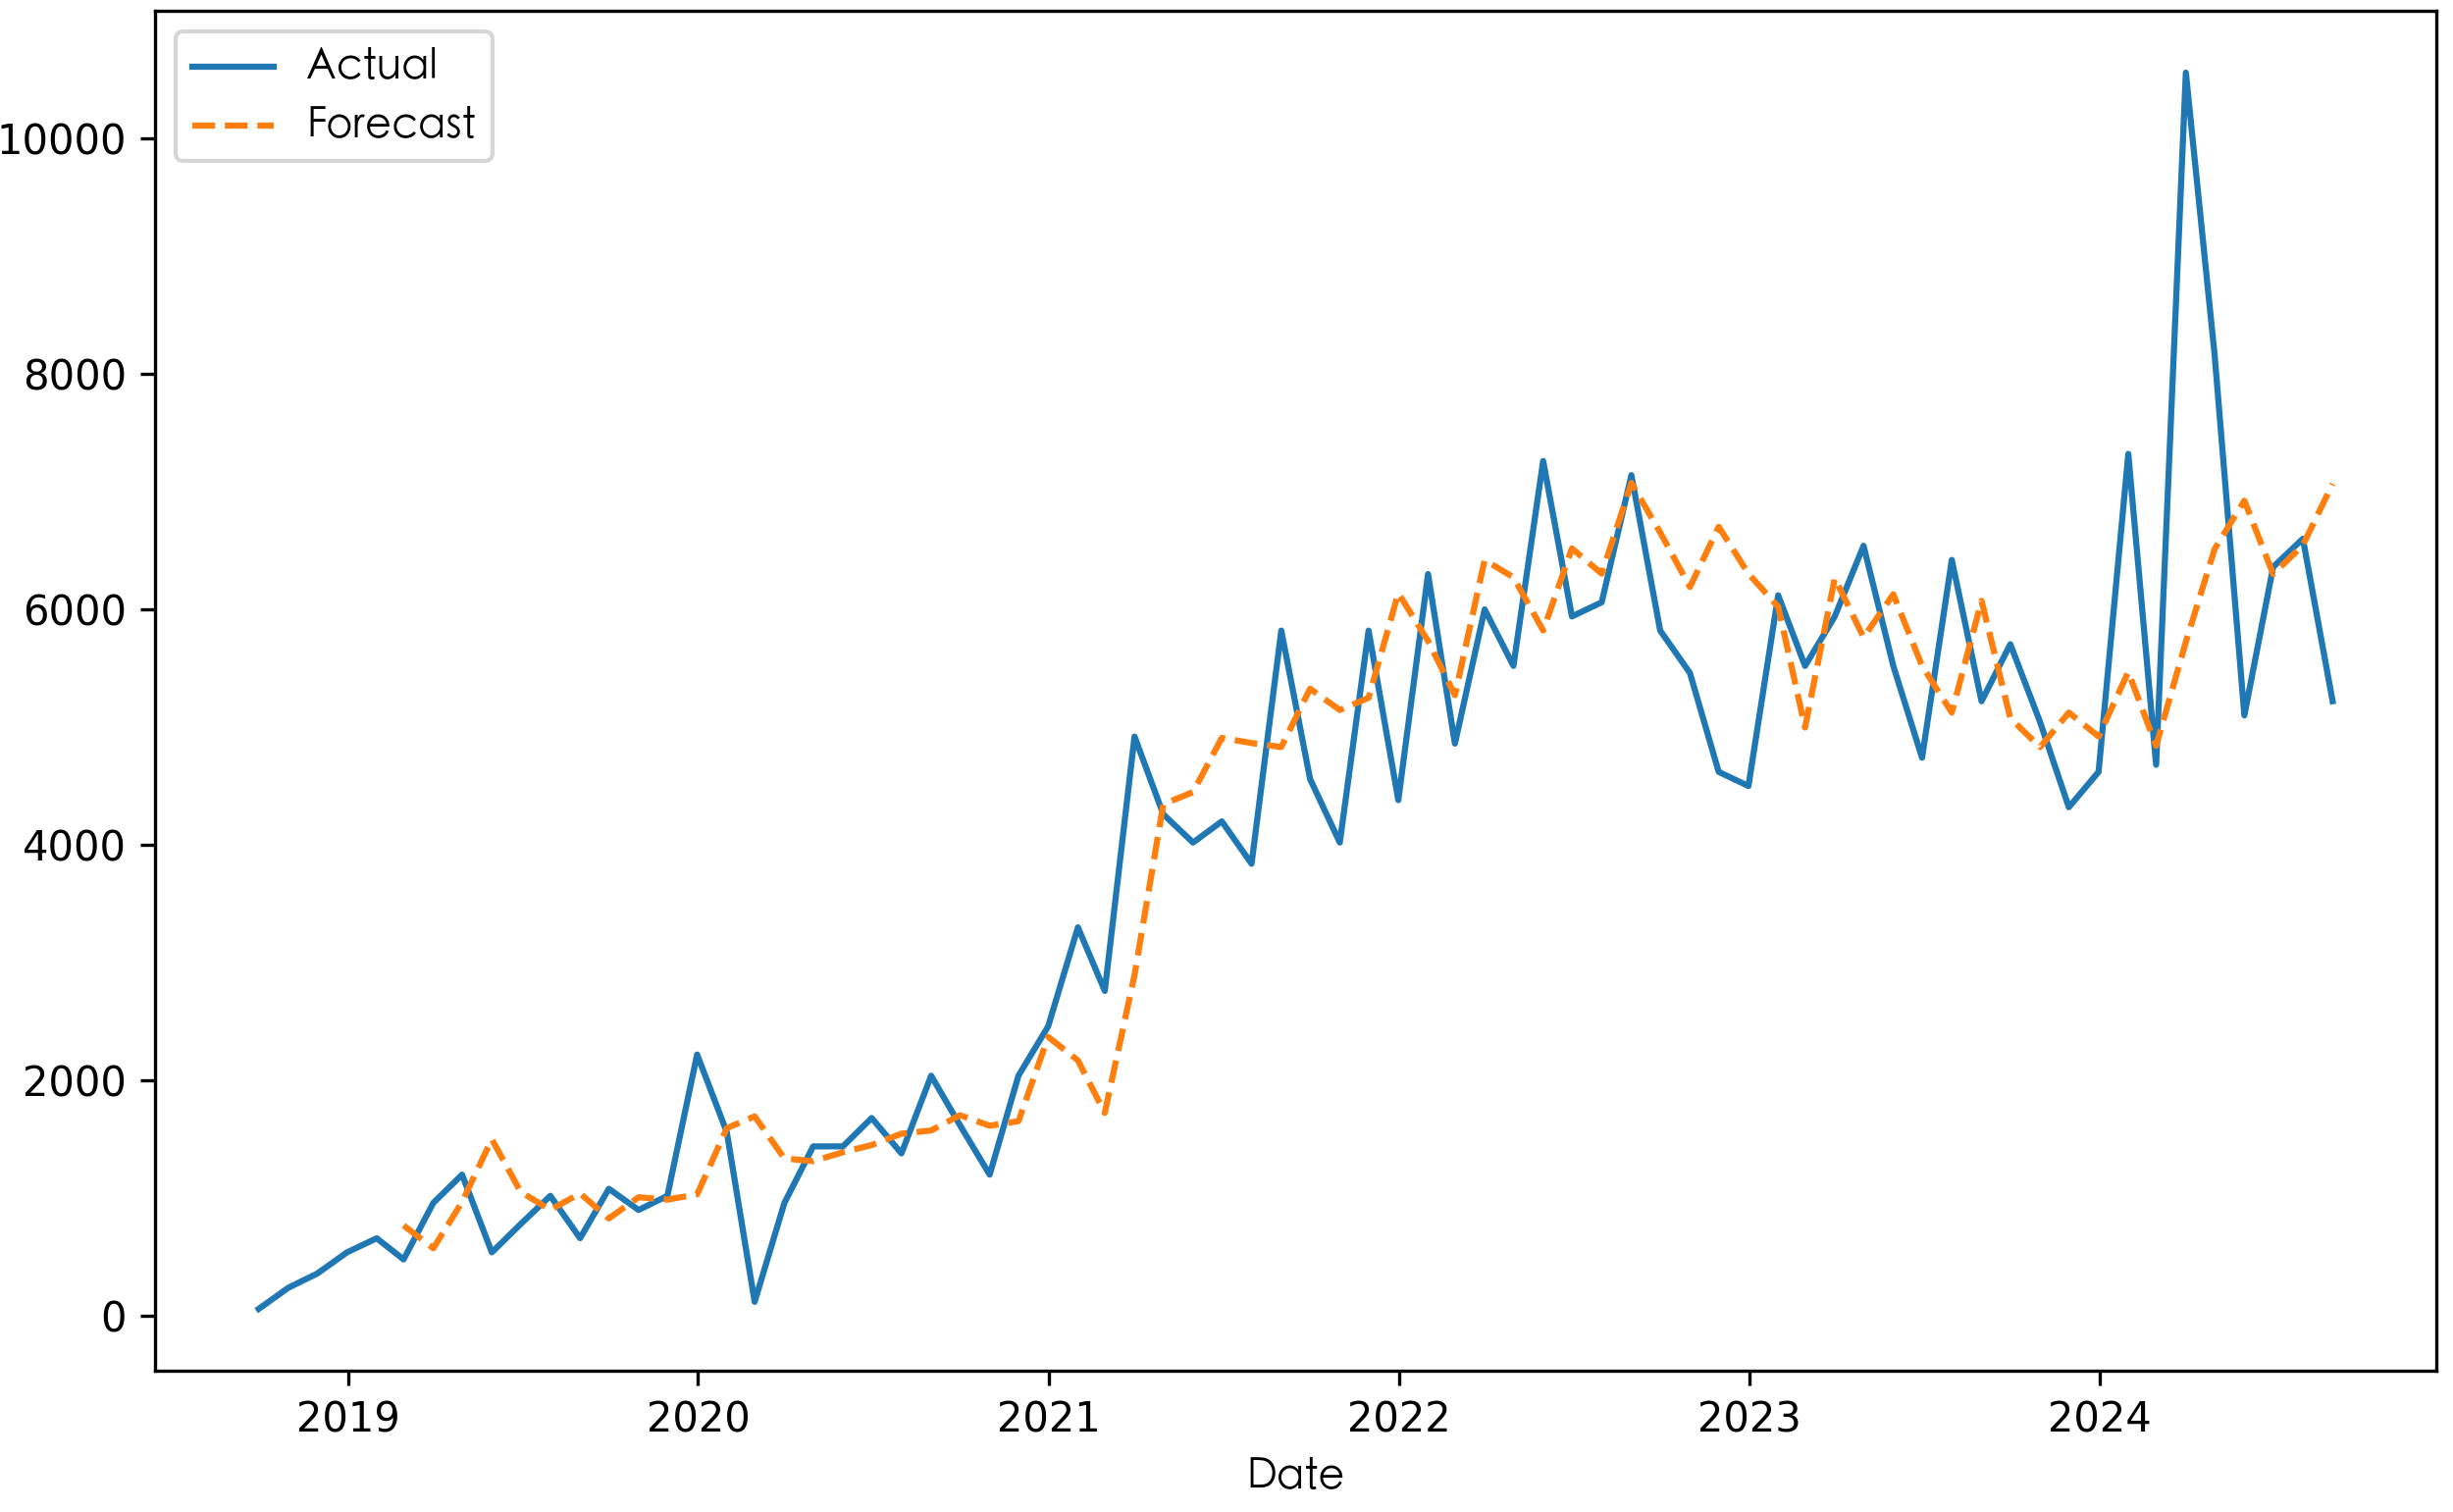
\includegraphics[width=\linewidth]{/Users/aprilwu/Desktop/Result_Paper/Prophet_Prediction_复方黄柏液涂剂_鲁汉方.png}
\caption{Prophet Prediction for Compound Phellodendron Liquid by Lu Hanfang.}
\label{fig:phellodendron}
\end{figure}
\item \textbf{Drug:} Shenshuaining Tablets
\begin{itemize}
\item \textbf{Manufacturer:} Shanhaiguan Pharmaceutical
\item \textbf{Metrics:} $R^2 = 0.7348$, RMSE = 1759.35, MAE = 1258.51, SMAPE = 21.86
\end{itemize}
Prophet's capability to handle multiple seasonality levels and trend changes made it the optimal choice for this drug's complex sales pattern.
\begin{figure}[H]
\centering
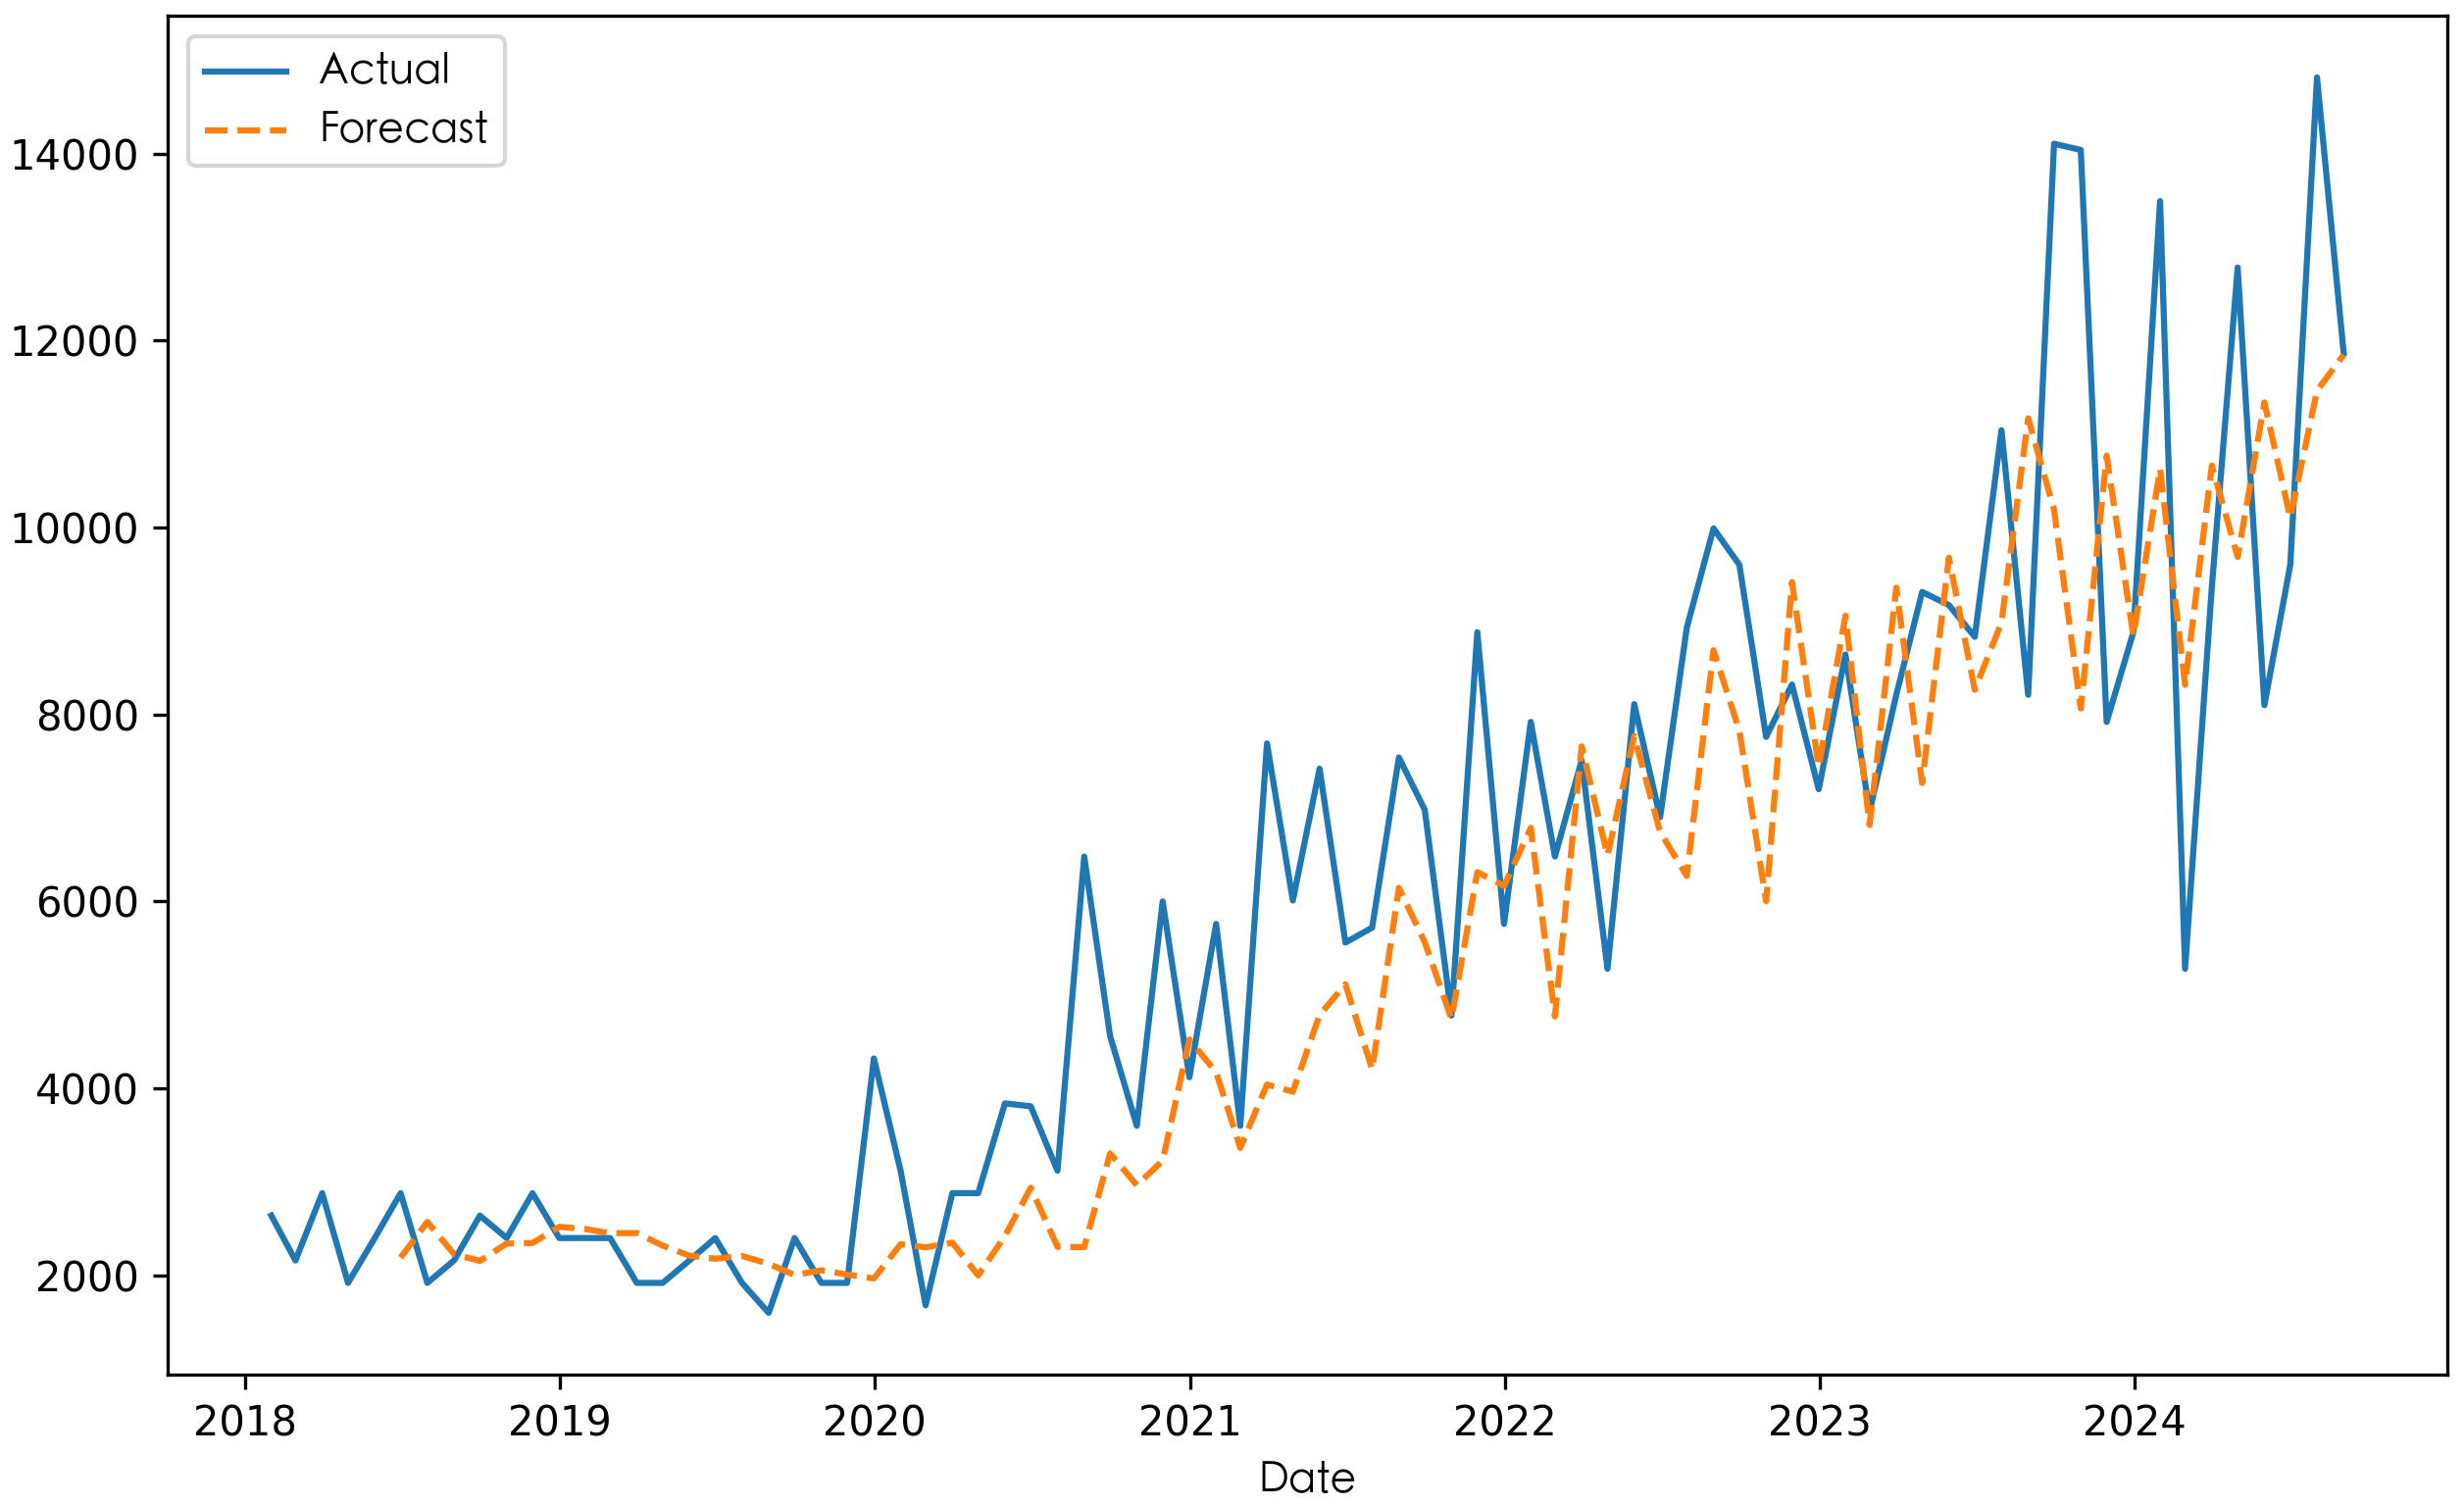
\includegraphics[width=\linewidth]{/Users/aprilwu/Desktop/Result_Paper/Prophet_Prediction_肾衰宁片_山海关药业.png}
\caption{Prophet Prediction for Shenshuaining Tablets by Shanhaiguan Pharmaceutical.}
\label{fig:shenshuaining}
\end{figure}
\end{itemize}

\paragraph{SARIMAX Model}
\begin{itemize}
\item \textbf{Drug:} Peritoneal Dialysis Solution [Lactate]
\begin{itemize}
\item \textbf{Manufacturer:} Huaren
\item \textbf{Metrics:} $R^2 = 0.8109$, RMSE = 1005.61, MAE = 661.08, SMAPE = 32.49
\end{itemize}
SARIMAX demonstrated superior performance for this drug due to its ability to capture both the seasonal patterns and the gradual decline in demand shown in the time series. The model effectively handled the relatively stable periodic fluctuations until the sharp decline in 2023.
\begin{figure}[H]
\centering
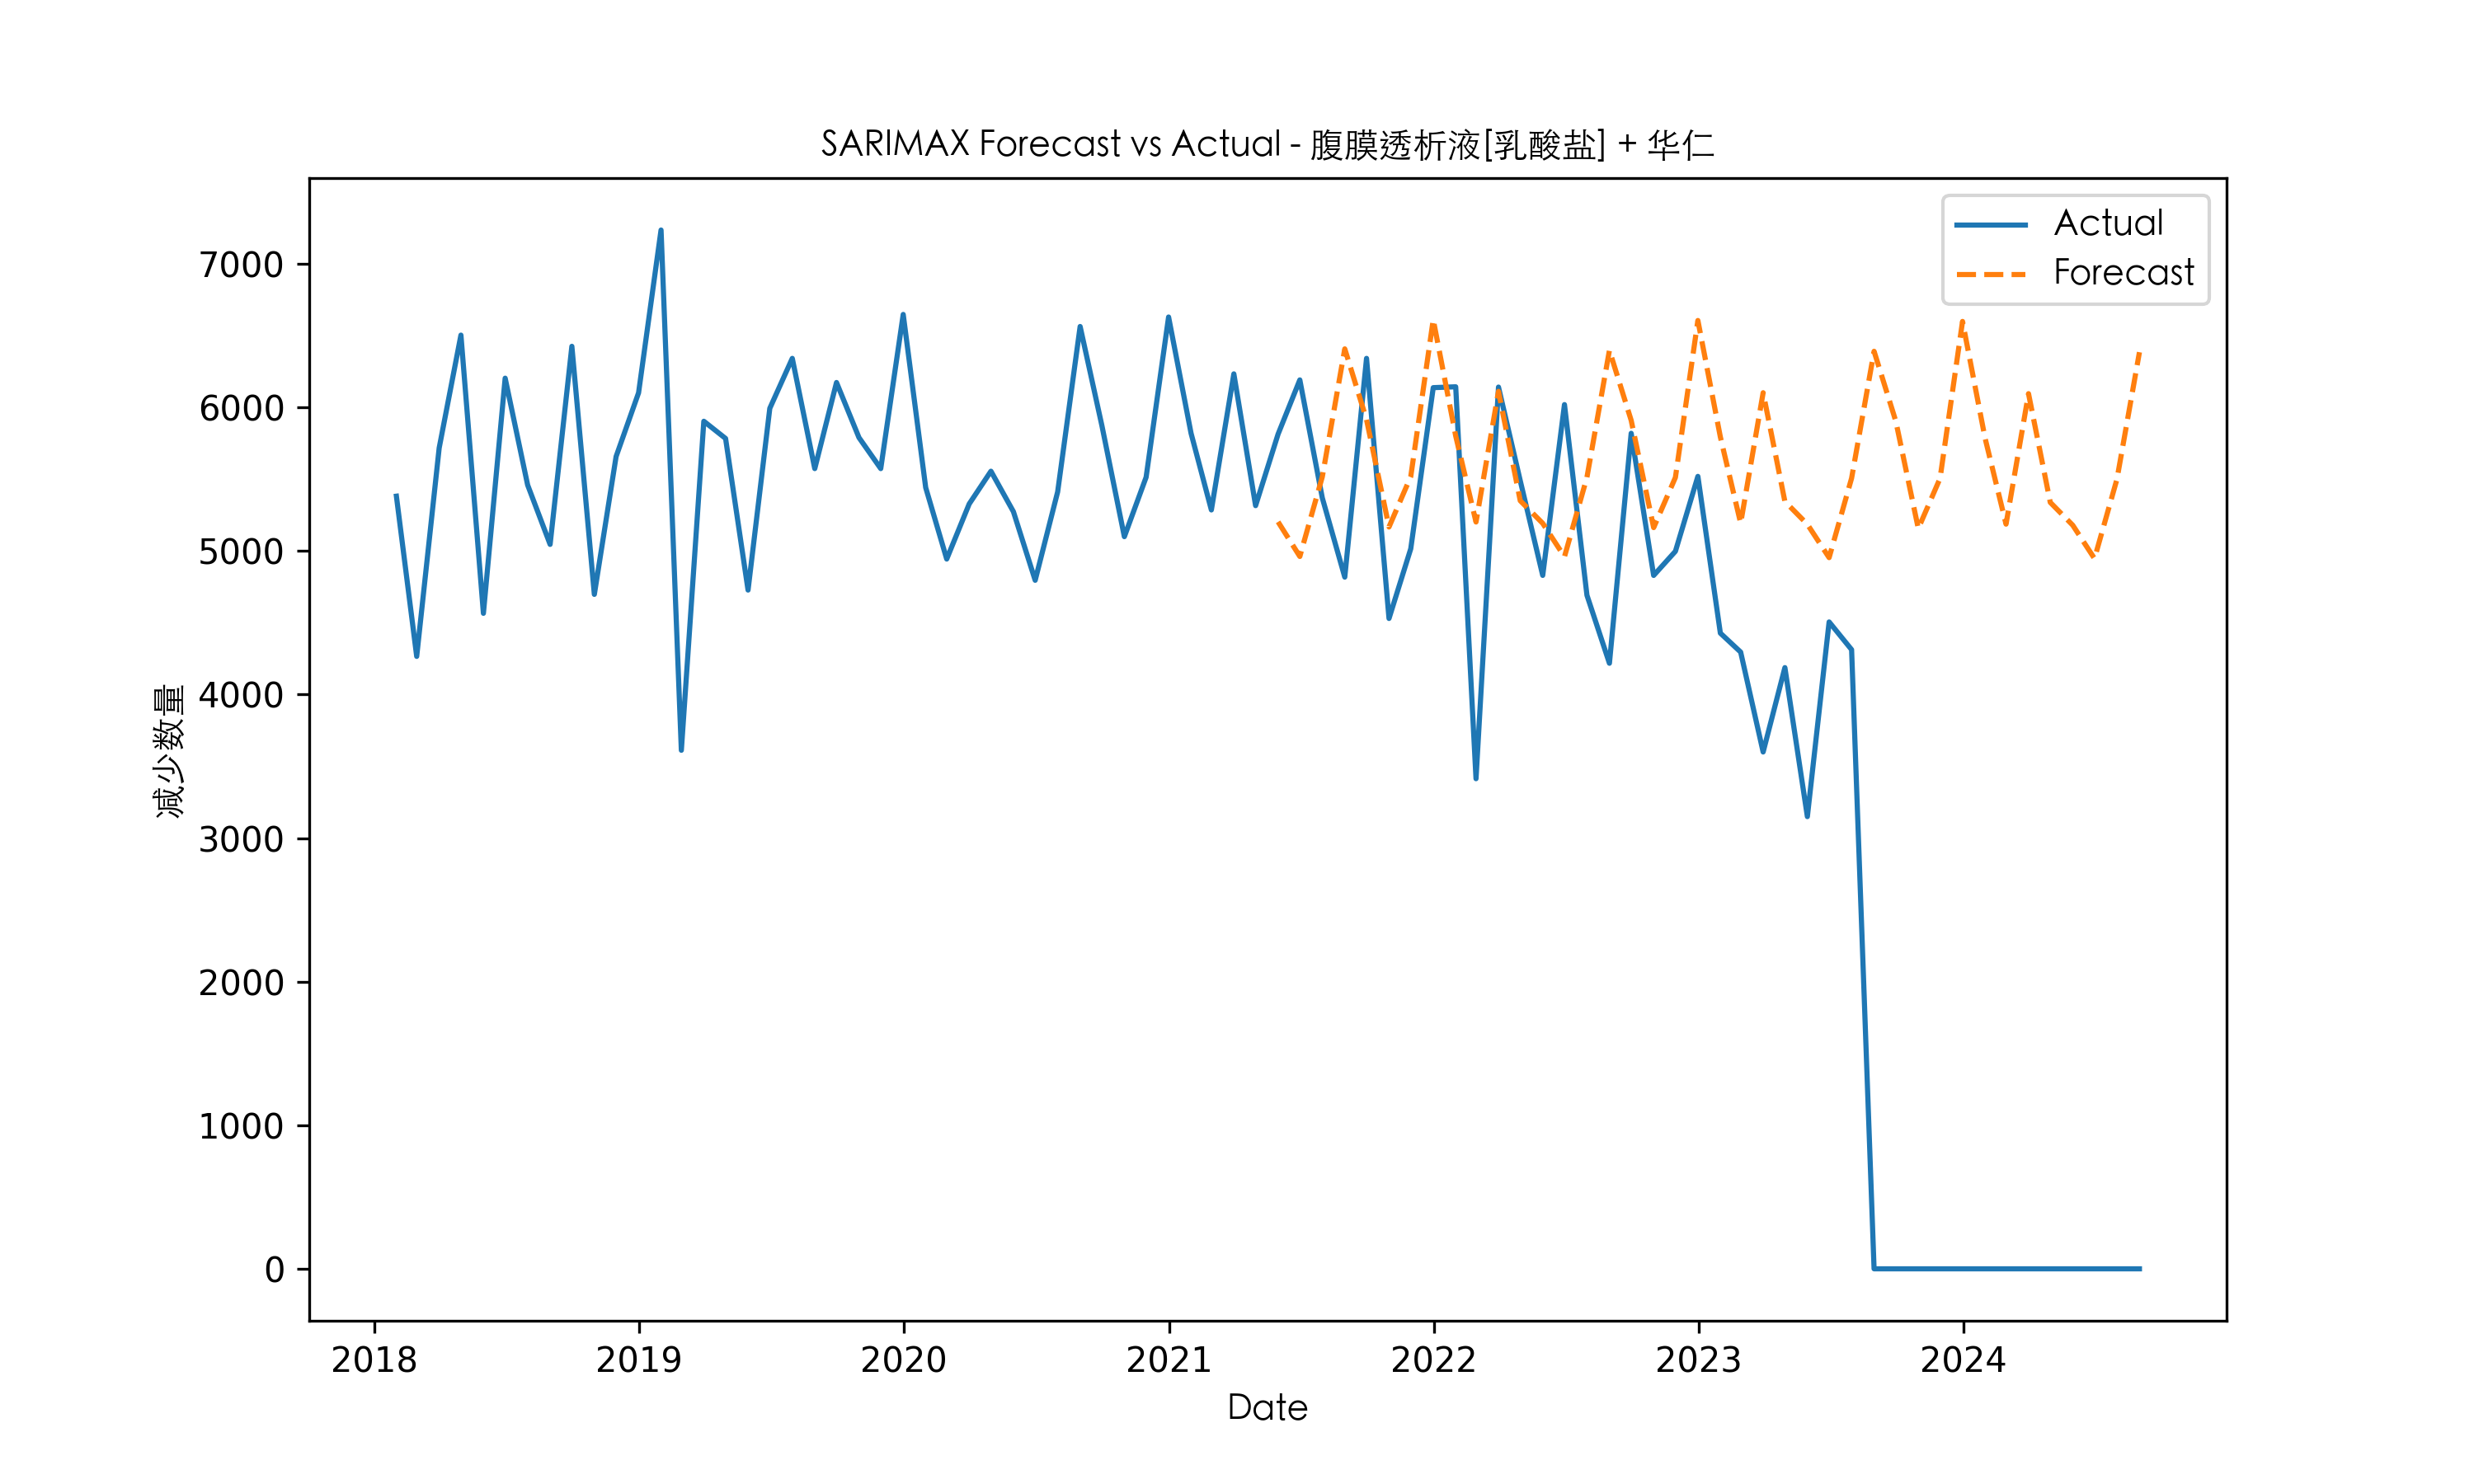
\includegraphics[width=\linewidth]{/Users/aprilwu/Desktop/Result_Paper/SARIMAX_Prediction_腹膜透析液[乳酸盐]_华仁.png}
\caption{SARIMAX Prediction for Peritoneal Dialysis Solution by Huaren.}
\label{fig:peritoneal}
\end{figure}
\item \textbf{Drug:} Vitamin B1 Tablets
\begin{itemize}
\item \textbf{Manufacturer:} Xinyi Huanghe
\item \textbf{Metrics:} $R^2 = 0.7345$, RMSE = 130.45, MAE = 87.49, SMAPE = 35.37
\end{itemize}
The SARIMAX model was particularly effective for this drug due to its ability to handle the regular seasonal patterns and moderate volatility in the sales data.
\begin{figure}[H]
\centering
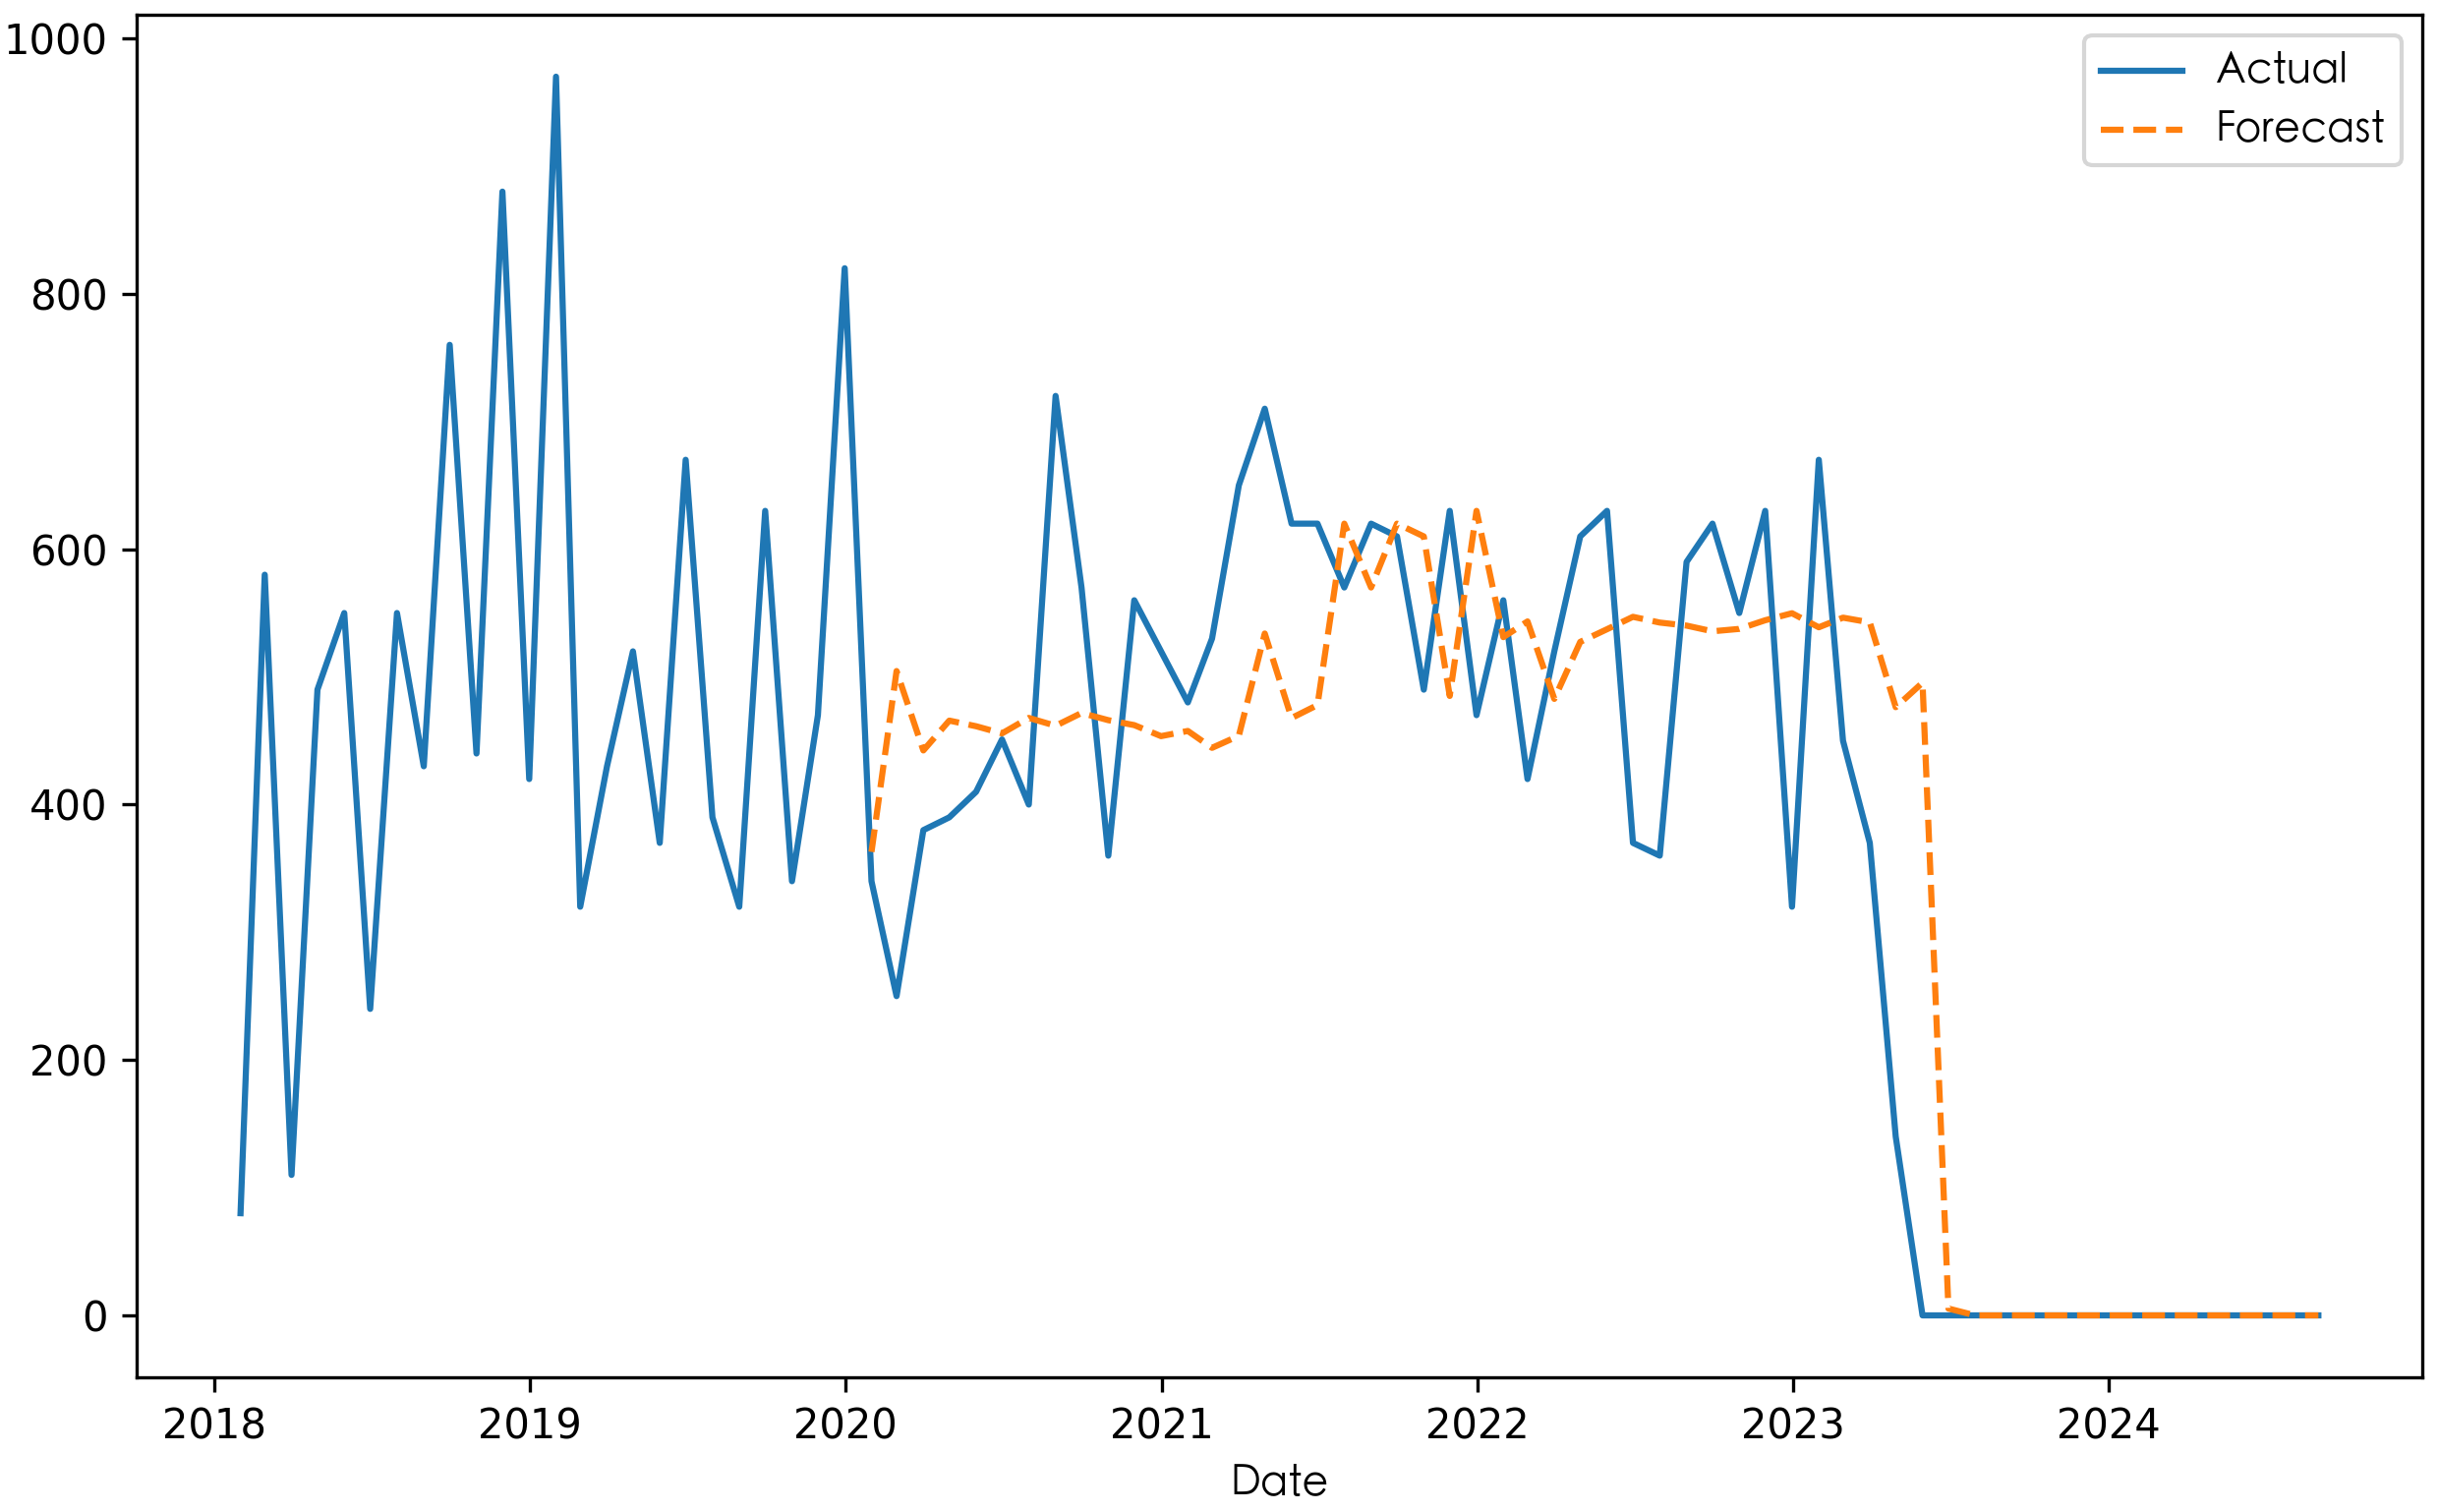
\includegraphics[width=\linewidth]{/Users/aprilwu/Desktop/Result_Paper/SARIMAX_Prediction_维生素B1片_信谊黄河.png}
\caption{SARIMAX Prediction for Vitamin B1 Tablets by Xinyi Huanghe.}
\label{fig:vitaminb1}
\end{figure}
\end{itemize}

\subsubsection{Overall Results}

Across all drug-manufacturer pairs, XGBoost emerged as the most frequently selected model, particularly for drugs with complex interactions and non-linear dynamics. SARIMAX was preferred for cases with strong seasonal patterns, while Prophet excelled in instances with irregular growth trends.

The selection process ensures that the optimal model was chosen for each combination, leveraging the unique strengths of each approach. By aligning model characteristics with data patterns, we minimized prediction errors and provided actionable forecasts.

The visualization analysis reveals several key findings:

\textbf{Long-term Trend Capture}:
\begin{itemize}
\item All models effectively captured the underlying growth trends, with Prophet showing particular strength in long-term pattern recognition.
\item SARIMAX demonstrated superior performance in capturing gradual trend changes, as evidenced in the insulin device forecasts.
\end{itemize}
\textbf{Seasonal Pattern Recognition}:
\begin{itemize}
\item XGBoost effectively captured complex seasonal patterns in chronic medication usage.
\item SARIMAX showed strong performance in regular seasonal variations, particularly in established products.
\end{itemize}
\textbf{Growth Pattern Adaptation}:
\begin{itemize}
\item Prophet demonstrated superior capability in adapting to emerging growth patterns.
\item XGBoost showed strong performance in capturing non-linear growth relationships.
\end{itemize}

These results highlight the robustness of the forecasting framework and its adaptability to diverse pharmaceutical sales scenarios. The chosen models’ ability to accurately predict future sales positions the framework as a valuable tool for strategic decision-making.


\subsection{Conclusion}
The results demonstrate the effectiveness of the hybrid framework in achieving robust and accurate forecasts across a diverse set of drug-manufacturer combinations. By tailoring model selection to the specific characteristics of each time series, we successfully leveraged the strengths of SARIMAX, Prophet, and XGBoost. The methodology provides a practical and adaptable solution for pharmaceutical demand forecasting, with potential applications in broader healthcare domains. Future work will focus on incorporating additional external variables and exploring ensemble techniques to further improve performance.

\section{Discussion and Future Work}
\subsection{Model Comparison and Hybrid Framework}
While each model has unique strengths and limitations, integrating their complementary capabilities within a hybrid framework provides significant advantages:

\begin{itemize}
    \item \textbf{XGBoost} handles nonlinear relationships effectively.
    \item \textbf{SARIMAX} captures seasonality and leverages external variables.
    \item \textbf{Prophet} provides robust decomposition of trend and seasonality.
\end{itemize}

The hybrid approach enables the framework to adapt to different data characteristics, achieving better overall prediction performance. For example, SARIMAX improves accuracy when seasonality dominates, whereas XGBoost captures complex interactions in data with dynamic patterns.

\subsection{Future Work}
To further improve drug inventory predictions, the following directions are proposed for future research:

\begin{itemize}
    \item \textbf{Hybrid Framework Expansion}: Extend the hybrid framework by integrating additional models, such as LightGBM, Transformer-based architectures, or ensemble methods to capture both short-term fluctuations and long-term trends.
    \item \textbf{External Variable Enrichment}: Explore additional exogenous variables such as patient inflow, epidemic outbreak data, seasonal illnesses (e.g., flu seasons), or hospital-specific factors to improve prediction accuracy.
    \item \textbf{Automated Model Selection}: Implement automated hyperparameter tuning and model selection techniques (e.g., Bayesian optimization) to improve forecasting performance with minimal manual intervention.
\end{itemize}

By addressing these areas, the proposed framework can become a more robust and scalable solution for hospital pharmacy inventory management, ensuring continuous patient care and reducing operational inefficiencies.

\section{Conclusion}
This study evaluated the performance of XGBoost, SARIMAX, and Prophet for drug inventory prediction in hospital pharmacies. The main findings are as follows:

\begin{itemize}
    \item XGBoost outperformed SARIMAX and Prophet in terms of RMSE and SMAPE for short-term predictions.
    \item SARIMAX demonstrated better performance when external (exogenous) variables were included and seasonal trends dominated the data.
    \item Prophet performed well in capturing long-term seasonality and trends but showed limitations in handling highly sparse data.
\end{itemize}

The hybrid framework, by combining these models, shows promise for improving prediction accuracy and robustness. Future work will focus on integrating real-time data streams and exploring additional hybrid models, such as Transformer-based architectures, to further enhance predictive capabilities.

\section{References}

\begin{thebibliography}{99}

    \bibitem{koala2021factors} 
    D. Koala, Z. Yahouni, G. Alpan, and Y. Frein, “Factors influencing drug consumption and prediction methods,” in \textit{CIGI-Qualita: Conférence Internationale Génie Industriel QUALITA}, Grenoble, France, 2021.
    
    \bibitem{taylor2018forecasting}
    S. J. Taylor and B. Letham, “Forecasting at scale,” \textit{The American Statistician}, vol. 72, no. 1, pp. 37–45, 2018.

    \bibitem{chen2016xgboost}
    T. Chen and C. Guestrin, “XGBoost: A scalable tree boosting system,” \textit{Proceedings of the 22nd ACM SIGKDD International Conference on Knowledge Discovery and Data Mining}, 2016, pp. 785–794.

    \bibitem{ferreira2018forecast}
    D. Ferreira, P. Teixeira, and A. Dias, “Exploring the performance of ARIMA and LSTM in time series forecasting: A comparative study,” \textit{International Journal of Computer Science and Applications}, vol. 15, no. 2, pp. 20–34, 2018.

    \bibitem{meng2021comparative}
    J. Meng, Q. Zhang, and X. Li, “Comparative analysis of Prophet and LSTM models in drug sales forecasting,” \textit{Journal of Physics: Conference Series}, vol. 1910, no. 1, p. 012059, 2021.

    \bibitem{xu2019hybrid}
    W. Xu, Y. Wang, and J. Zhao, “A hybrid modelling method for time series forecasting based on a linear regression model and deep learning,” \textit{Applied Intelligence}, vol. 49, no. 7, pp. 2875–2888, 2019.

    \bibitem{siddiqui2021hybrid}
    R. Siddiqui, A. Khan, and M. Ahmed, “A Hybrid Demand Forecasting Model for Greater Forecasting Accuracy: The Case of the Pharmaceutical Industry,” \textit{Supply Chain Forum: An International Journal}, vol. 22, no. 3, pp. 1–13, 2021.

    \bibitem{rathipriya2022pharma}
    R. Rathipriya, M. Saranya, and K. Ramkumar, “Demand Forecasting Model for Time-Series Pharmaceutical Data Using Neural Networks,” \textit{Neural Computing and Applications}, vol. 35, pp. 1945–1957, 2022.

\end{thebibliography}

\appendix
\section{Sample Selection Algorithm}
\label{appendix:sample-selection}

The following pseudocode outlines the sample selection process used to ensure the quality and relevance of the dataset for modeling tasks:

\begin{algorithm}[H]
\caption{Sample Selection Algorithm}
\begin{algorithmic}[1]
\Require Cleaned data $df$, configuration thresholds $\text{config}$
\Ensure Filtered dataset $final\_df$
\State $final\_df \gets \emptyset$
\For{each unique combination of drug name and manufacturer $(d, m)$ in $df$}
    \State $group\_data \gets$ subset of $df$ for $(d, m)$
    \If{length of $group\_data < \text{config.min\_months}$ \textbf{or} sum of consumption $= 0$}
        \State \textbf{Skip group} \Comment{Insufficient or sparse data}
    \EndIf
    \State $non\_zero\_ratio \gets$ proportion of non-zero consumption in $group\_data$
    \If{$non\_zero\_ratio < \text{config.sparsity\_threshold}$}
        \State \textbf{Skip group} \Comment{Data too sparse}
    \EndIf
    \State $acf\_values \gets$ autocorrelation function of consumption in $group\_data$
    \If{$\max(acf\_values[1:]) < \text{config.min\_acf\_threshold}$}
        \State \textbf{Skip group} \Comment{Insufficient autocorrelation}
    \EndIf
    \If{no start date $\geq \text{config.min\_start\_date}$ in $group\_data$}
        \State \textbf{Skip group} \Comment{No recent data}
    \EndIf
    \State $variance \gets$ variance of consumption in $group\_data$
    \If{$variance < \text{config.min\_variance\_threshold}$}
        \State \textbf{Skip group} \Comment{Variance too low}
    \EndIf
    \State $missing\_ratio \gets$ maximum missing ratio for features in $group\_data$
    \If{$missing\_ratio > \text{config.max\_missing\_ratio}$}
        \State \textbf{Skip group} \Comment{Feature missing data too high}
    \EndIf
    \State $skewness \gets$ skewness of consumption in $group\_data$
    \If{$|skewness| > \text{config.max\_skewness}$}
        \State \textbf{Skip group} \Comment{Target variable too skewed}
    \EndIf
    \State $correlation \gets$ correlation of consumption with lagged features in $group\_data$
    \If{$|correlation| < \text{config.min\_correlation}$}
        \State \textbf{Skip group} \Comment{Insufficient correlation with features}
    \EndIf
    \State $final\_df \gets final\_df \cup group\_data$
\EndFor
\State \Return $final\_df$
\end{algorithmic}
\end{algorithm}

\bibliographystyle{IEEEtran}
\bibliography{references}

\end{document}
